\documentclass[../../index.tex]{subfiles}

\begin{document}
\chapter{Introduction}
In particle physics we are concerned about small objects and their interactions.
Since the 1970 the dynamics of these tiny pieces are best described by the Standard Model (SM).

The SM contains two groups of fermionic, Spin 1/2 particles. The former group,
the leptons consist of: the electron ($e$), the muon ($\mu$), the tau ($\tau$)
and their corresponding neutrinos $\nu_e$, $\nu_\mu$ and $\nu_\tau$. The latter
group, the quarks contain: $u$, $d$ (up and down, the so called light quarks ),
$s$ (strange), $c$ (charm), $b$ (bottom or beauty) and $t$ (top or truth). The SM
furthermore differentiates between three fundamental forces (and its carriers):
the electromagnetic ($\gamma$ photon), weak ($Z$\-/ or $W$\-/Boson) and strong ($g$
gluon) interactions. The before mentioned Leptons solely interact through the
electromagnetic and the weak force (also referred to as electroweak interaction),
whereas the quarks additionally interact through the strong force. A short
summary of the taxonomy of the SM can be seen in \cref{fig:SMTaxonomy}
\begin{figure}
  \centering
  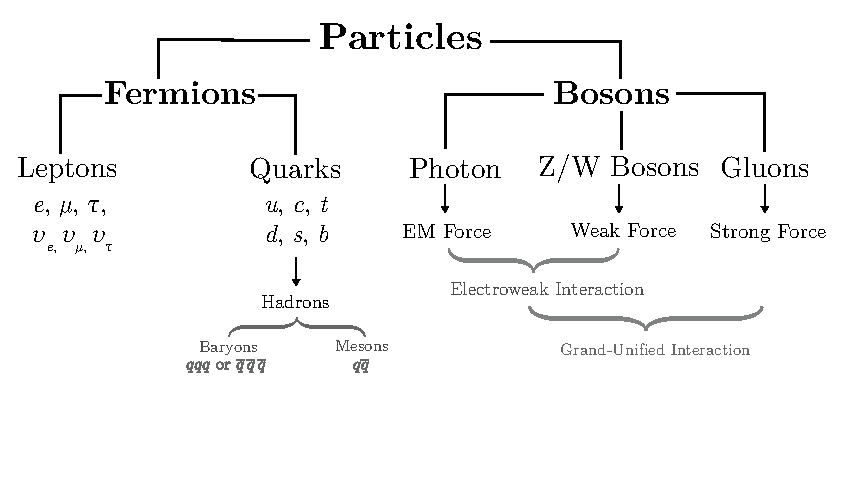
\includegraphics[width=\textwidth]{./images/standardModelTaxonomy.eps}
  \caption{Taxonomy of the Standard Model.}
  \label{fig:SMTaxonomy}
\end{figure}

All of the particles and forces given in the SM are described by a Lagrangian
containing 19 parameters. The parameters are represented by ten masses, four CKM\-/matrix parameters, the QCD\-/vacuum
angle, the Higgs\-/vacuum expectation value and three gauge coupling constants.
Every single parameter has to be fitted from experimental data. Highly accurate
values with low errors are crucial for theoretical calculated predictions. One
of the major error inputs of every theoretical output are uncertainties in these
parameters. In this work we will focus on one of the parameters, namely the
strong coupling $\alpha_s$, which forms part of the theory of
\textit{quantum chromodynamics} (QCD).

As the name suggest\footnote{Chromo is the Greek word for color.} QCD
is characterized by the color charge. Every quark has next to its type one
of the three colors blue, red or green. The color force is mediated through
eight gluons, which each being bi\-/colored\footnote{Each gluon carries a color
  and an anti\-/color.}, interact with quarks and each other. The strength of the
strong force is given by the coupling constant $\alpha_s$. The strong coupling
depends on the renormalization scale $\mu$, which is often chosen in a way that
the coupling constant $\alpha_s(q)$ depends on the energy $q^2$. Thus the
coupling varies with energy with an exceptional property: it increases for
low energies\footnote{In contrast to the electromagnetic force, where $\alpha(q^2)$
  decreases!}. This is exclusive for QCD and has two main implications.

The first one states, that for low energies the coupling is too strong for
isolate quarks to exist. Until now we have not been able to observe an isolated
quark and all experiments can only measure quark compositions. These bound
states are called \textit{hadrons} and consist of two or three quarks
\footnote{There exist also so\-/called \textit{Exotic hadrons}, which have more
  than three valence quarks.}, which are referred to as mesons\footnote{Composite
  of a quark and an anti\-/quark.} or baryons \footnote{Composite of three quarks
  or three anti\-/quarks.} respectively. This
phenomenon, of quarks sticking together as hadrons is referred to as \textit{confinement}. 
As the fundamental degrees of freedom of QCD are given by quarks and gluons, but
the observed particles are hadrons we need to introduce the assumption of
\textit{quark\-/hadron duality} to match the theory to the experiment. This means that a physical quantity should be
similarly describable in the hadronic picture or quark\-/gluon picture and that
both descriptions are equivalent. As we will see in our work quark\-/hadron
duality is violated for low energies. These so\-/called \textit{duality
  violations} have an impact on our strong coupling determinations and can be
dealt with either suppression or the inclusion of a model
\cite{Pich2006,Cata2008}.
Throughout this work we will favor and argument for the former approach.

The second implication concerns \textit{perturbation theory} (PT). The lower
the energies we deal with, the higher the value of the strong coupling and the
contributions of \textit{non\-/perturbative} (NP) effects. Currently there are
three solutions to deal with NP effects:
\begin{itemize}
  \item \textbf{\textit{Chiral Perturbation Theory}} (ChPT): Introduced by Weinberg
    \cite{Weinberg1978} in the late seventies. ChPT is an effective field theory
    constructed with a Lagrangian symmetric under chiral transformation in the
    limit of massless quarks. It's limitations are based in the chiral symmetry,
    which is only a good approximation for the light quarks $u$, $d$ and in some
    cases $s$.
  \item \textbf{\textit{Lattice QCD}} (LQCD): Is the numerical approach to the strong
    force. Based on the Wilson Loops \cite{Wilson1974} we treat QCD on a finite
    lattice instead of working with continuous fields. LQCD has already many applications but
    is limited due to its computational expensive calculations.
  \item \textbf{\textit{QCD Sum Rules}} (QCDSR): Was also introduced in the late seventies by
    Shifman, Vainstein and Zakharov \cite{Shifman1978,Shifman1978a}. It relates
    the observed hadronic picture to quark\-/gluon parameters through a dispersion
    relation and the use of the \textit{Operator Product Expansion} (OPE), which
    treats NP effect through the definition of vacuum expectation values, the
    so\-/called \textit{QCD condensates}. It is a precise method for extracting
    the strong coupling $\alpha_s$ at low energies, although limited to
    the unknown higher order contributions of the OPE.
\end{itemize}

In this work we focus on the determination of the strong coupling $\alpha_s$
within the framework of QCD Sum Rules for $\tau$\-/decays which has been
exploited in the beginning of the nineties by Braaten, Narison and Pich \cite{Braaten1991}. Within this setup we
can measure $\alpha_s(m_\tau^2)$ at the $m_\tau$ scale. As the strong coupling
gets smaller at higher energies, so do the errors. Thus if we obtain the strong
coupling at a low scale we will obtain high precision values at the scale of the
Z\-/boson mass $m_Z$, which is the standard scale to compare $\alpha_s$ values.

The QCDSR for the determination of $\alpha_s$, from low energies, contain three major issues.
\begin{enumerate}
  \item There are two different approaches to treat perturbative and non\-/perturbative
contributions. In particular, there is a significant difference between results
obtained using fixed\-/order (FOPT) or contour improved perturbation theory
(CIPT), such that analyses based on CIPT generally arrive at about 7\% larger
values of $\alpha_s(m_{\tau^2})$ than those based on FOPT \cite{PDG2018}.
There have been a variety of analyses on the topic been performed
\cite{Pich2013,Caprini2009,Jamin2005} and we will favor the FOPT approach,
but generously list our results for the CIPT framework.

  \item There are several prescriptions to deal with the NP-contributions of
    higher order OPE condensates. Typically terms of higher dimension have been
    neglected, even if they knowingly contribute. In this work we will include
    every necessary OPE term.

  \item Finally there are known DV leading to an ongoing discussion of the
importance of contributions from DV. Currently there are two main approaches:
Either we neglect them, arguing that they are sufficiently suppressed due to
\textit{pinched weights} \cite{Pich2016} or model DV with sinusoidal
exponentially suppressed function \cite{Cata2008,Boito2011,Boito2014} introducing
extra fitting parameters. We will argue for the former method, implementing
pinched weights that sufficiently suppress DV contributions such as having only a negligible effect on our analysis.
\end{enumerate}

In the first chapter of this work we want to summarize the necessary theoretical
background for working with the QCDSR. Starting with the basics of QCD we want to motivate the
\textit{renormalization group equation} (RGE), which is responsible for the
running of the strong coupling. We then continue with the some
aspects of the two\-/point function and its usage in the dispersion relation,
which connects the hadronic picture with the quark\-/gluon picture. $\cdots$

\end{document}